\documentclass[crop,tikz]{standalone} 
\usepackage{tikz, amsmath, amssymb, graphicx} 

\DeclareMathAlphabet\mathbfcal{OMS}{cmsy}{b}{n}

\newcommand{\Mt}{\mathbfcal{M}}
\newcommand{\Yt}{\mathbfcal{Y}}
\newcommand{\Ft}{\mathbfcal{F}}

\usetikzlibrary{positioning, shapes.geometric} 

\begin{document} 

\begin{tikzpicture}


\node[inner sep=0pt] at (0, 1.9) {Time};
\node [draw, red, dashed, shape=rectangle, minimum width=1.2cm, minimum height=3cm, anchor=center] at (0,0) {};
\node[inner sep=0pt] at (0, 0) {$t$};
\node[inner sep=0pt] at (0, -1.9) {$429$};


\node [opacity=0, text opacity=1] at (1, 0) {$\otimes$};
\node [opacity=0, text opacity=1] at (1, -1.9) {$\times$};


\node[inner sep=0pt] at (3, 1.9) {Use of funds};
\node [draw, green, dashed, shape=rectangle, minimum width=3.2cm, minimum height=3cm, anchor=center] at (3,0) {};
\node [opacity=0, text opacity=1] at (3, 0) {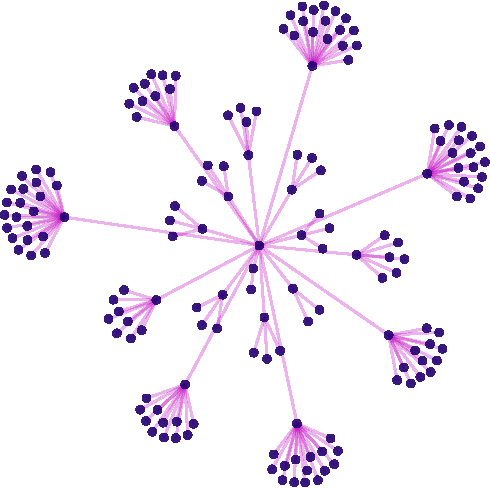
\includegraphics[width=.23\textwidth]{bond_graph_small.pdf}};
\node[inner sep=0pt] at (3, -1.9) {$161$};

\node [opacity=0, text opacity=1] at (5, 0) {$\otimes$};
\node [opacity=0, text opacity=1] at (5, -1.9) {$\times$};

\node[inner sep=0pt] at (6, 1.9) {Rating};
\node [draw, blue, dashed, shape=rectangle, minimum width=1.2cm, minimum height=3cm, anchor=center] at (6,0) {};
\node[inner sep=0pt] (AAA) at (6, 1) {AAA};
\node[inner sep=0pt] (AA+) at (6, 0.4) {AA+};
\node[inner sep=0pt] (AA+) at (6, -0.2) {$\vdots$};
\node[inner sep=0pt] (AA+) at (6, -1) {BBB+};
\node[inner sep=0pt] at (6, -1.9) {$8$};

\node [opacity=0, text opacity=1] at (7, 0) {$\otimes$};
\node [opacity=0, text opacity=1] at (7, -1.9) {$\times$};


\node[inner sep=0pt] at (8, 1.9) {Maturity};
\node [draw, orange, dashed, shape=rectangle, minimum width=1.2cm, minimum height=3cm, anchor=center] at (8,0) {};
\node[inner sep=0pt] (AAA) at (8, 1) {30-50y};
\node[inner sep=0pt] (AA+) at (8, 0.4) {20-30y};
\node[inner sep=0pt] (AA+) at (8, -0.2) {$\vdots$};
\node[inner sep=0pt] (AA+) at (8, -1) {0-1y};
\node[inner sep=0pt] at (8, -1.9) {$8$};

\node [opacity=0, text opacity=1] at (9, 0) {$\otimes$};
\node [opacity=0, text opacity=1] at (9, -1.9) {$\times$};


\node[inner sep=0pt] at (10.5, 1.9) {Tax status};
\node [draw, cyan, dashed, shape=rectangle, minimum width=2cm, minimum height=3cm, anchor=center] at (10.5,0) {};
\node[inner sep=0pt] (AAA) at (10.5, 0) {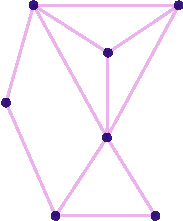
\includegraphics[width=.13\textwidth]{tax_graph_small.pdf}};
\node[inner sep=0pt] at (10.5, -1.9) {$7$};

% \draw [green, dashed] (1, -2.7) rectangle (2.05, 0.3);

% \node [below, opacity=0, text opacity=1] at (2.45, -1) {$\otimes$};

% \draw [blue, dashed] (2.9, -2.7) rectangle (6.5, 0.3);
% \node[inner sep=0pt] (subjects) at (6.2, -0.2) {};

% \node [below, opacity=0, text opacity=1] at (6.9, -1) {$\otimes$};

% \draw [orange, dashed] (7.4, -2.7) rectangle (10.5, 0.3);
% \node[inner sep=0pt] (stimuli) at (10.3, -0.2) {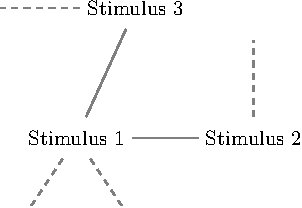
\includegraphics[width=.22\textwidth]{fMRI_Stimuli_Diagram.pdf}};




\end{tikzpicture}
\end{document} 
